\documentclass{article}
\usepackage[utf8]{inputenc}
\usepackage{graphicx}
\usepackage{hyperref}
\hypersetup{
    colorlinks,
    citecolor=black,
    filecolor=black,
    linkcolor=black,
    urlcolor=black
}
\graphicspath{ {Flowcharts/images/} }
\title{\Huge{\textbf{Lab 6 \\* Flow Free}\textsuperscript{\small\textregistered}
                        \\*  CSE 379 \\* Introduction To \\* Microprocessors}}
\date{} %remove date from make title


\begin{document}
    \pdfbookmark[1]{Title Page}{title}
    \maketitle
    \vfill 
    {\Large\centering\textbf{Jesse Both \\* Nicholas Anzalone}\par}
    {\large\centering{Lab Section: R1}\par}
    {\large\centering{\today}\par}
    \newpage
    \pdfbookmark[1]{Table of Contents}{TOC}
    \begin{center}
        \tableofcontents
    \end{center}
\newpage
\setcounter{secnumdepth}{-1}


\section{Program Overview}
The purpose of this program was to implement the game
Flow Free in ARM Assembly. Some of the major tasks include:

    \begin{itemize}
        \item utilizing the UART0, SW2 and LED 
        \item breaking the correct links when links are crossed 
        \item determining the correct link character that should be displayed
        \item determining when to increment or decrement completed
        \item outputing a random board 
        \item hiding the board when the game is paused
    \end{itemize}

\subsection{Division of Work}
-
\subsubsection{Jesse}
    Implemented the main functionality of the game.
\subsubsection{Nick}
    Implemented the functionality such as the random
    board, pause screen and timer.


\newpage
\section{Subroutines}
-

\subsection{Lab6.s}
    This file does a lot of miscellaneous tasks, but a major part of it
    is how the link coordinates are stored. Each color has 30 available bytes
    in memory to place coordinates. The reason 30 was chosen is because it is 
    the maximum number of links that needs to be stored (+starting O). The links
    are stored like this:
    \begin{center}
        {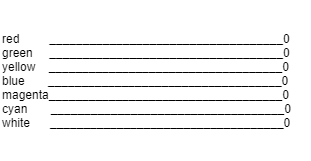
\includegraphics[height=3cm]{links.png}\centering} 
    \end{center}
    \subsubsection{lab6}
        This is the main routine of the program.  It initializes everything 
        and print the title screen to Putty.  It then loops until an interrupt
        happens.
        \begin{center}
            {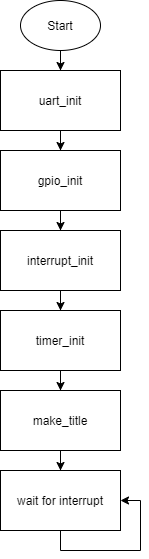
\includegraphics[height=8cm]{lab6.png}\centering} 
        \end{center}
        \newpage

    \subsubsection{init\_game}
        This routine sets up the game to be played.  First it resets everything
        then it prints all the necessary elements of the game to Putty.
        \begin{center}
            {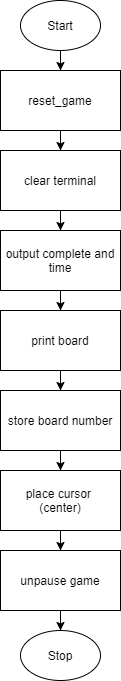
\includegraphics[height=9cm]{init_game.png}\centering} 
        \end{center}
        \newpage

    \subsubsection{reset\_game}
        This subroutine resets each element of the game. It removes all
        links, turns off led and sets the timer and completed to 0
        \begin{center}
            {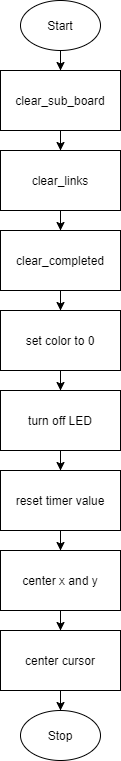
\includegraphics[height=10cm]{reset_game.png}\centering} 
        \end{center}
        \newpage

    \subsubsection{move\_cursor}
        This subroutine is responsible for moving the cursor after WASD is pressed.
        It increments the cursor coordinates to move relative to the key that was
        pressed
        \begin{center}
            {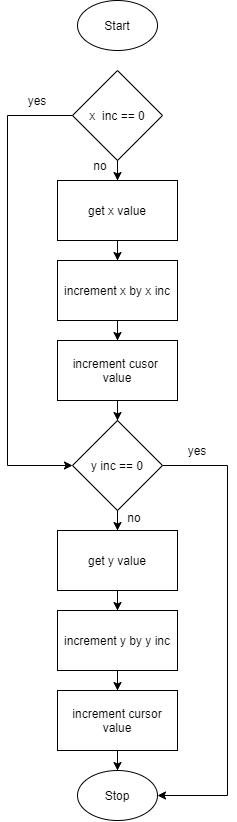
\includegraphics[height=10cm]{move_cursor.png}\centering} 
        \end{center}
    
    \subsubsection{put\_time}
        This subroutine places the correct updated time to the correct
        position on the screen.
        \begin{center}
            {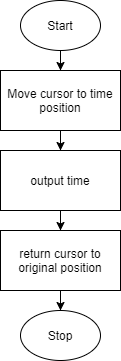
\includegraphics[height=5cm]{put_time.png}\centering} 
        \end{center}
        \newpage

    \subsubsection{place\_text}
        This subroutine receives the inputs of a char and cursor pointer.
        First it places the char in the correct position in the string.
        It then moves the cursor to the input position and prints the char
        in that location.  The cursor is restored to its previous position.
        \begin{center}
            {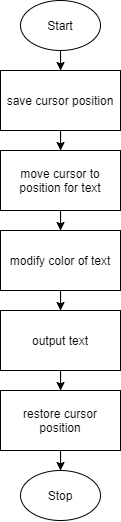
\includegraphics[height=7cm]{place_text.png}\centering} 
        \end{center}
    
    \subsubsection{color\_text}
        This subroutine takes a input of 0-7 for the new color.
        It converts the int to char and places it in the foreground 
        position.
        \begin{center}
            {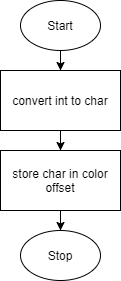
\includegraphics[height=4cm]{color_text.png}\centering} 
        \end{center}
        \newpage

    \subsubsection{modify\_cursor\_two}
        This routine changes the x and y values of cursor\_two. This relies on
        the other subroutine get\_cursor\_pos to get those x and y values
        \begin{center}
            {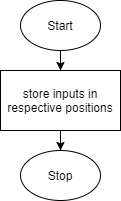
\includegraphics[height=3.5cm]{modify_cursor_two.png}\centering} 
        \end{center}
        
    \subsubsection{timer\_to\_string}
        This routine takes in an int for the timer and converts it it to 
        the correct ansi string that it needs to be placed in the correct position
        of the screen.
        \begin{center}
            {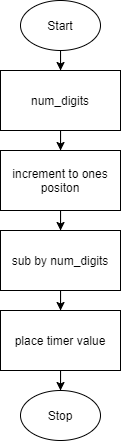
\includegraphics[height=7cm]{timer_to_string.png}\centering} 
        \end{center}
        \newpage

    \subsubsection{store\_pos}
        This subroutine has inputs for x, y and the current active color.
        It then stores the coordinates in memory as a byte at the end of 
        the colors space.
        \begin{center}
            {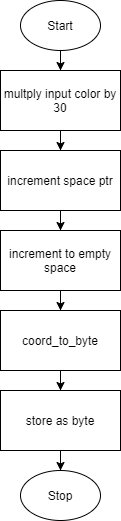
\includegraphics[height=8cm]{store_pos.png}\centering} 
        \end{center}
        \newpage

    \subsubsection{show\_link}
        This subroutine is responsible for placing the correct link
        on the board in the correct location.  Its input is a color
        to determine what color the link should be.
        \begin{center}
            {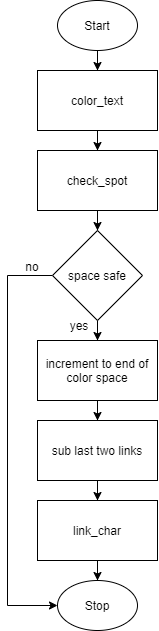
\includegraphics[height=9cm]{show_link.png}\centering} 
        \end{center}
        \newpage

    \subsubsection{link\_char}
        This subroutine determines what the correct type of link is
        required.  It returns a '+', '-' or 'I'
        \begin{center}
            {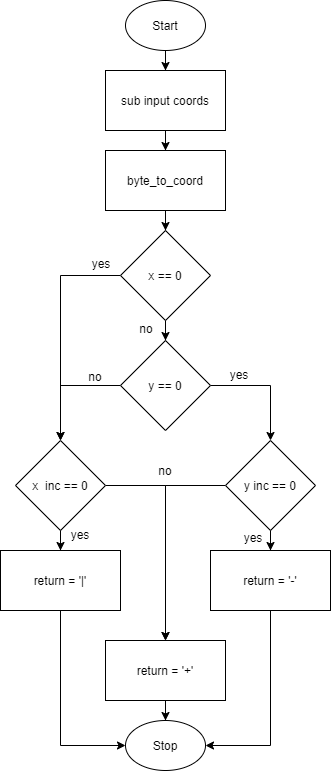
\includegraphics[height=10cm]{link_char.png}\centering} 
        \end{center}
        \newpage

    \subsubsection{show\_plus}
        This subroutine outputs a plus in the current position.
        This is used when space is pressed to deactivate the links.
        \begin{center}
            {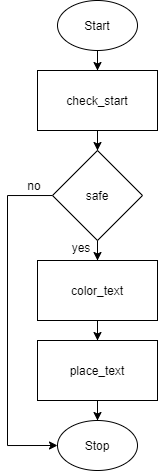
\includegraphics[height=8cm]{show_plus.png}\centering} 
        \end{center}
        
    \subsubsection{clear\_links}
        This subroutine clears all the link coordinates from memory.
        This is used to to within reset\_game.
        \begin{center}
            {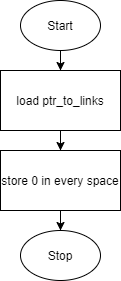
\includegraphics[height=5cm]{clear_links.png}\centering} 
        \end{center}
        \newpage   

    \subsubsection{clear\_color\_links}
        This subroutine clears all the links of a specific color.  
        This routine is used when a link is already started and
        an O is selected.
        \begin{center}
            {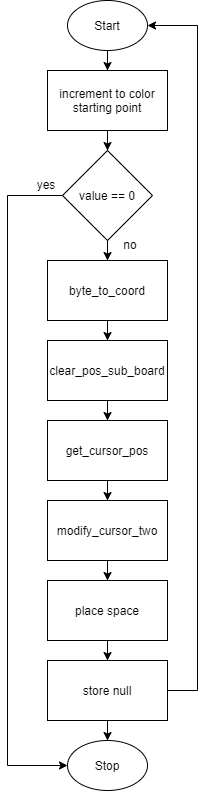
\includegraphics[height=10cm]{clear_color_links.png}\centering} 
        \end{center}
        \newpage
        
    
    \subsubsection{clear\_pos\_links}
        This subroutine takes in the color of links that needs to be broken.
        It uses the current x and y coordinates to determine where to start 
        breaking the links.  Once it finds those coordinates it breaks all
        the links after it for that specific color.
        \begin{center}
            {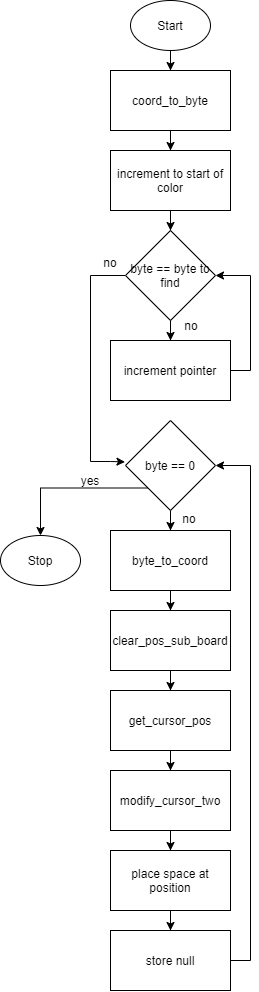
\includegraphics[height=12cm]{clear_pos_links.png}\centering} 
        \end{center}
        \newpage

    \subsubsection{replace\_links}
        This routine is used when the game is unpaused.  Due to poor planning
        each link has to be recalculated to determine what char should be used
        in the link.
        \begin{center}
            {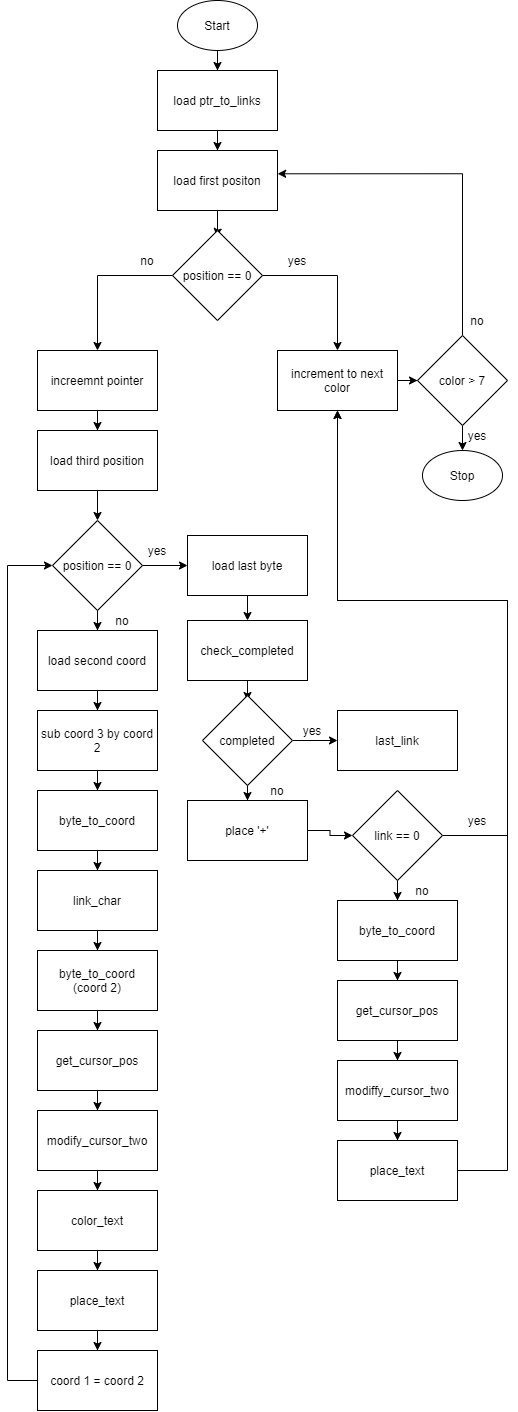
\includegraphics[height=14cm]{replace_links.png}\centering} 
        \end{center}
        \newpage
        
    \subsubsection{check\_start}
        This subroutine determines if the O that the cursor is currently 
        on was the start link or an end link. Its input is the current
        active color.
        \begin{center}
            {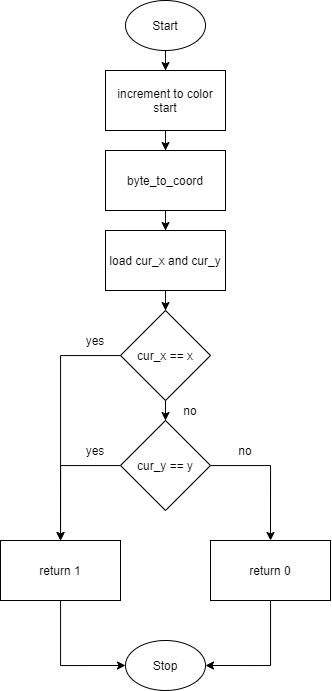
\includegraphics[height=10cm]{check_start.png}\centering} 
        \end{center}
        \newpage

    \subsubsection{Timer\_Handler}
        This interrupt handler is responsible for incrementing the timer
        when the game is not paused.
        \begin{center}
            {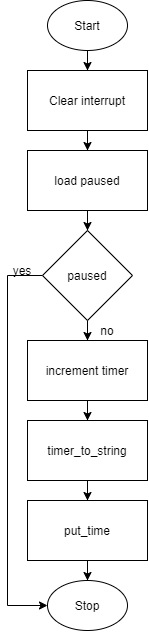
\includegraphics[height=9cm]{Timer_Handler.png}\centering} 
        \end{center}
        \newpage   

    \subsubsection{Switch\_Handler}
        This interrupt handler is responsible for pausing and unpausing
        the game when it is able.
        \begin{center}
            {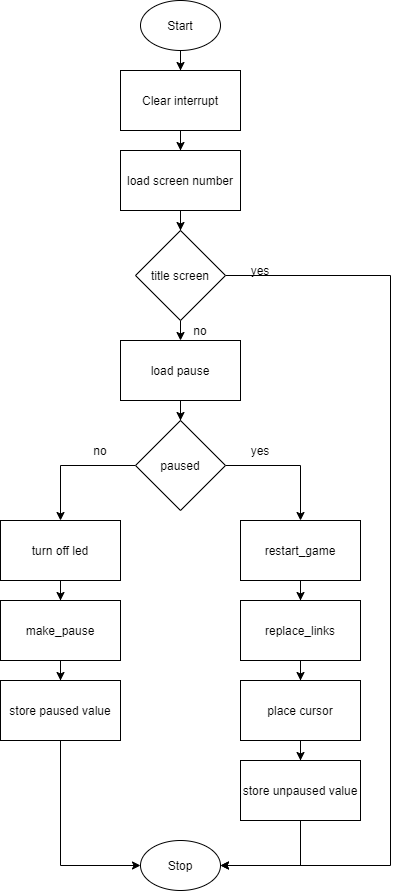
\includegraphics[height=12cm]{Switch_Handler.png}\centering} 
        \end{center}
        \newpage   


    \subsubsection{UART0\_Handler}
        This interrupt handler is responsible for all key presses within
        the game.  It does what ever operation is necessary regaurding 
        moving, making links, breaking links, triggering a completed link and triggering
        a completed board.
        \begin{center}
            {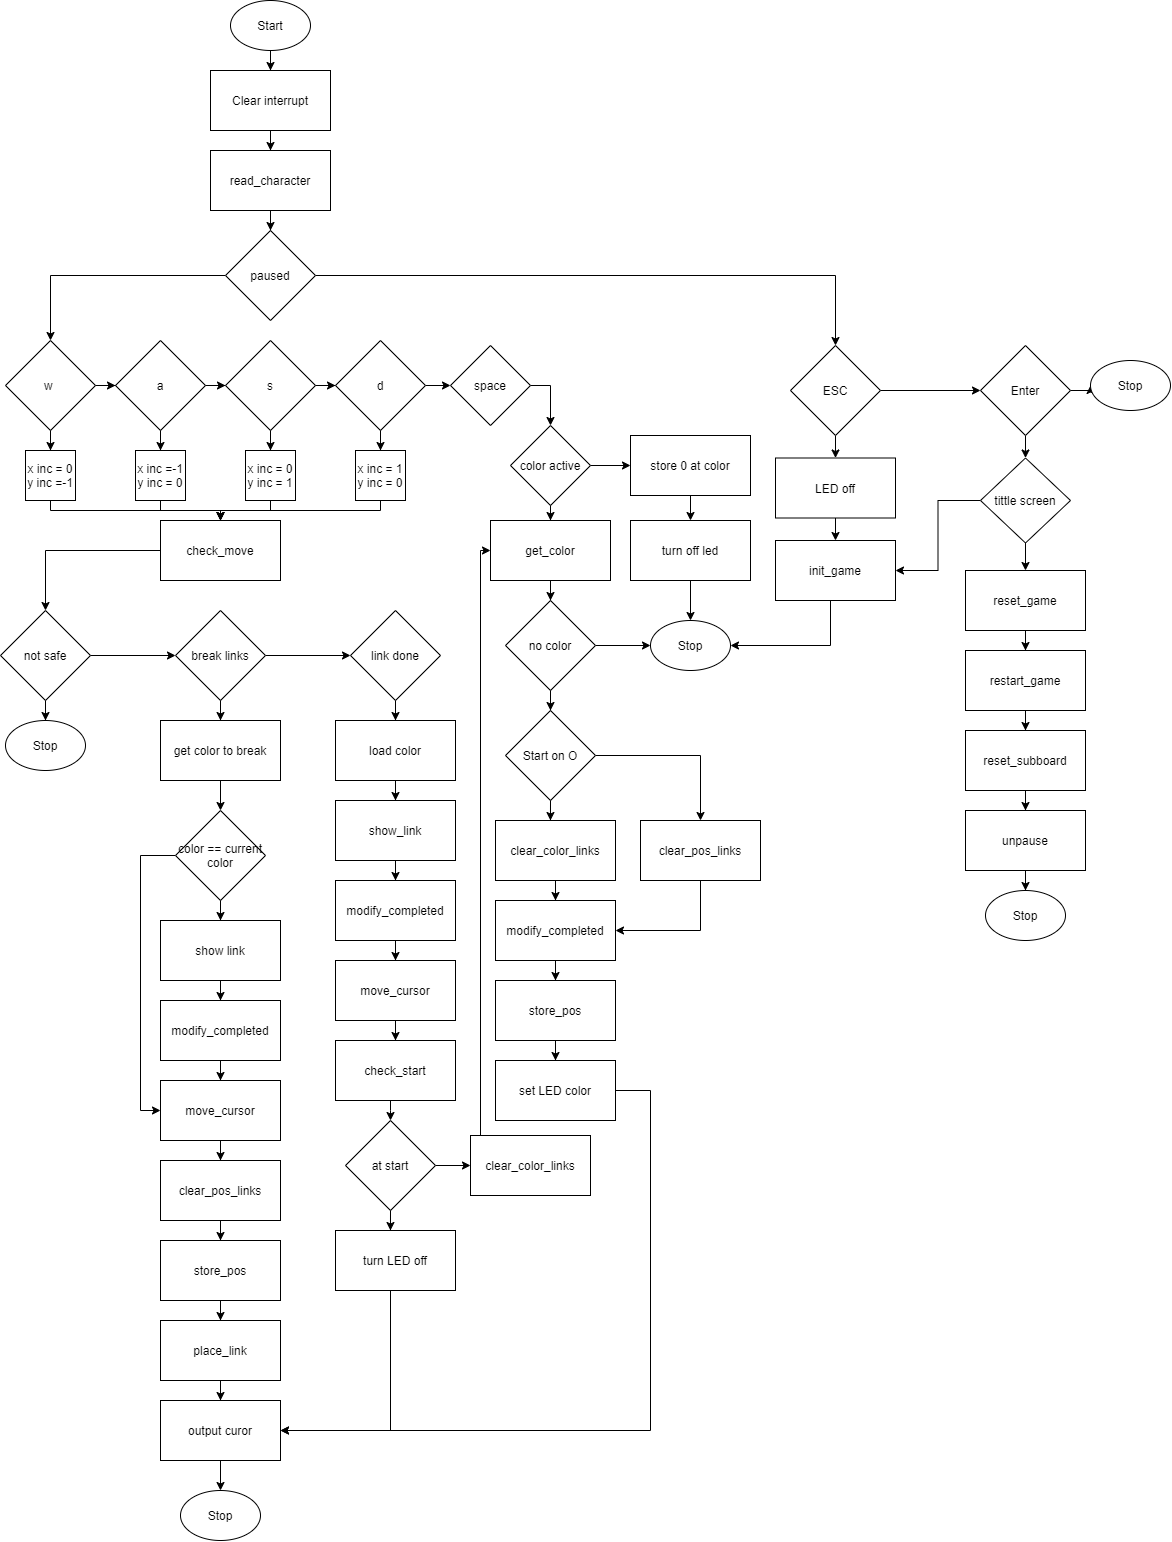
\includegraphics[height=16cm]{UART0_Handler.png}\centering} 
        \end{center}
        \newpage   
  
        
\subsection{Title.s}
    This file does is responsible for changing the screen to
    the title screen, end screen or pause screen.
    \subsubsection{make\_title}
        This routine will create the title menu that is to be displayed while the game first starts and 
        print that menu to the screen.
        \begin{center}
            {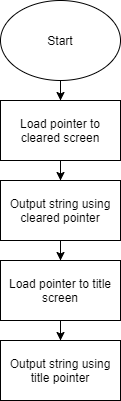
\includegraphics[height=6cm]{make_title.png}\centering} 
        \end{center}
        \newpage

    \subsubsection{make\_pause}
        This routine will create the pause menu that is to be displayed while the game is paused and 
        print that menu to the screen.
        \begin{center}
            {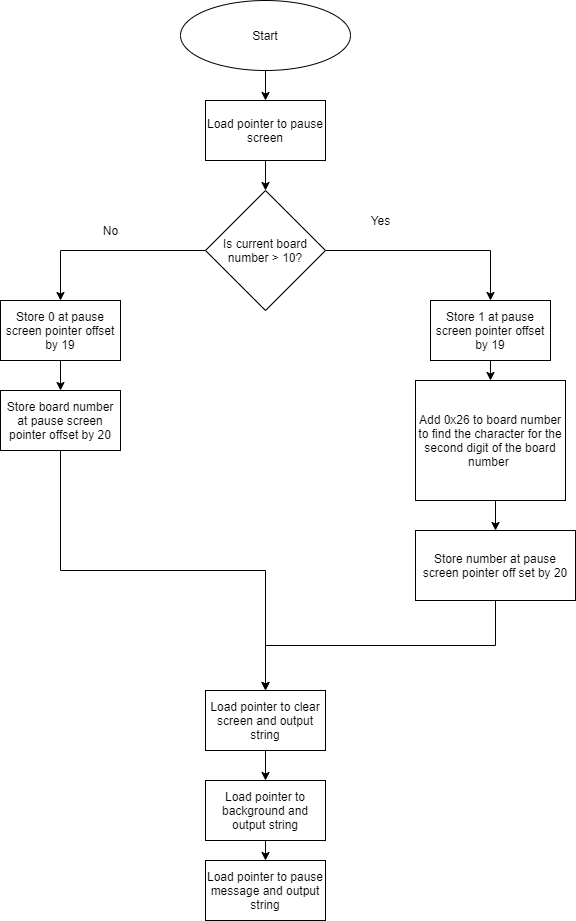
\includegraphics[height=11cm]{make_pause.png}\centering} 
        \end{center}

    \newpage
    \subsubsection{make\_end}
        This routine will create the end game menu that is to be displayed when a game has been socessfully
        completed.
        \begin{center}
            {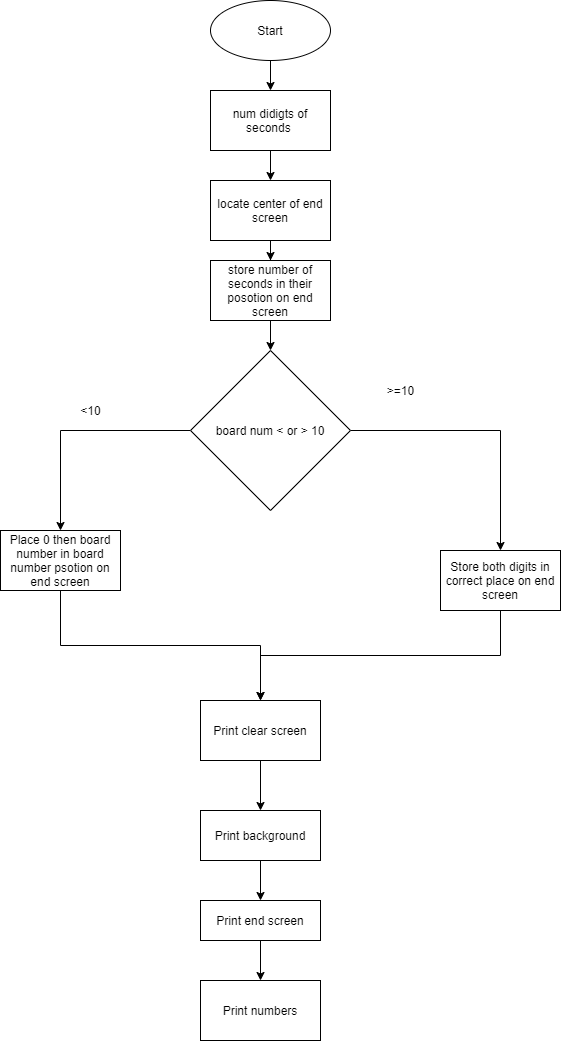
\includegraphics[height=14cm]{make_end.png}\centering} 
        \end{center}

    \newpage


\subsection{Board.s}
        The purpose of this file is to do the board output operations. This is 
        where the random board is determined. Each boards string is in memory 
        like so:
        \begin{center}
            {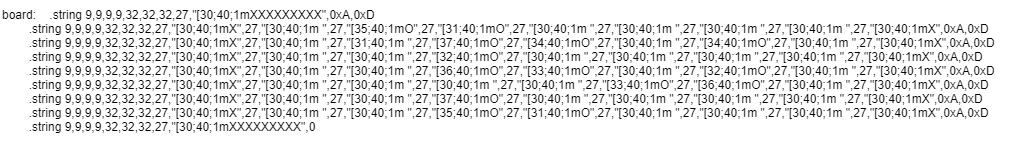
\includegraphics[height=2cm]{board.png}\centering} 
        \end{center}
    \subsubsection{board\_out}
        This routine chooses a random board from boards 1-16, and prints the board to the screen.
        In order to generate the random number, the value from the internal timer is pulled and the
        first bit from the timer is isolated. Effectivley randomly generating a number 1-16.
        \begin{center}
            {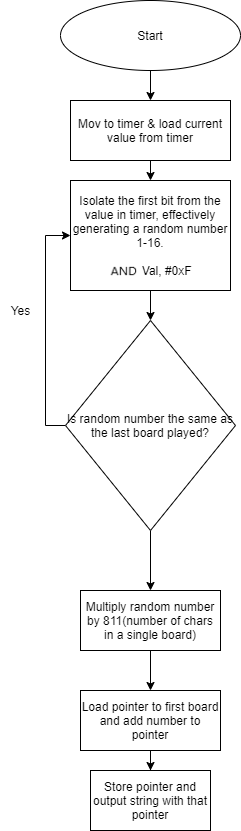
\includegraphics[height=10cm]{board_out.png}\centering} 
        \end{center}
        \newpage

    \subsubsection{reprint\_board}
        This routine prints out the current board in the current state it is in. It is used when going from
        paused state to unpaused state.
        \begin{center}
            {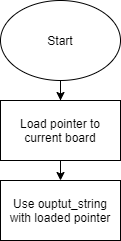
\includegraphics[height=3.5cm]{reprint_board.png}\centering} 
        \end{center}

    \subsubsection{reset\_subboard}
        This routine will reset the sub board to a clear sub board with no links. 
        This can be used when restarting a level.
        \begin{center}
            {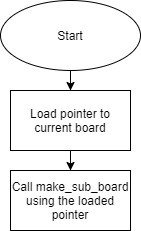
\includegraphics[height=3.5cm]{reset_subboard.png}\centering} 
        \end{center}

    \newpage


\subsection{Subboard.s}
        The purpose of this file is to simplify the board and remove
        all of the ansi characters from the board string.  How the 
        board looks is seen below.
        \begin{center}
            {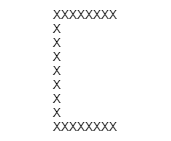
\includegraphics[height=4cm]{subboard.png}\centering} 
        \end{center}
    \subsubsection{make\_sub\_board}
        This subroutine converts the board string into a more
        manageable size.  The purpose of the subboard is to remove
        all ansi characters.
        \begin{center}
            {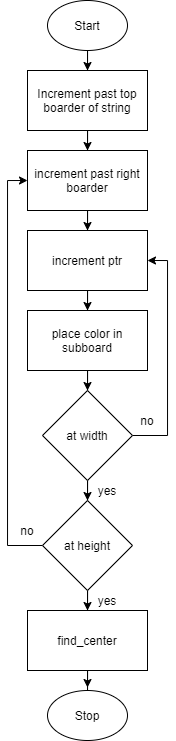
\includegraphics[height=11cm]{make_sub_board.png}\centering} 
        \end{center}
        \newpage

    \subsubsection{test\_sub\_board}
        This routine was used to test that the subboard was doing what
        it was supposed to.

    \subsubsection{find\_center}
        The subroutine incrments the subboards ptr to the center
        position to be used in rouines like check\_move.
        \begin{center}
            {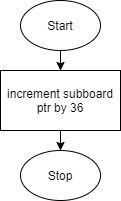
\includegraphics[height=3cm]{find_center.png}\centering} 
        \end{center}

    \subsubsection{clear\_sub\_board}
        This subroutine clears the subboard to its default state.
        \begin{center}
            {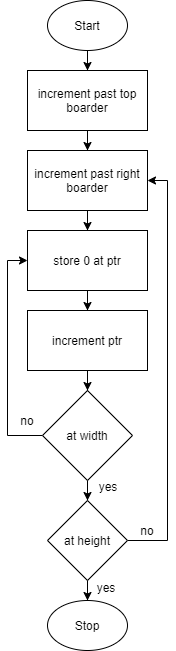
\includegraphics[height=10cm]{clear_sub_board.png}\centering} 
        \end{center}
        \newpage 
        
    \subsubsection{check\_move}
        This routine determines if the move is 'safe'. It also 
        is responsible for telling the program if links need to 
        be broken of if the link is completed.
        \begin{center}
            {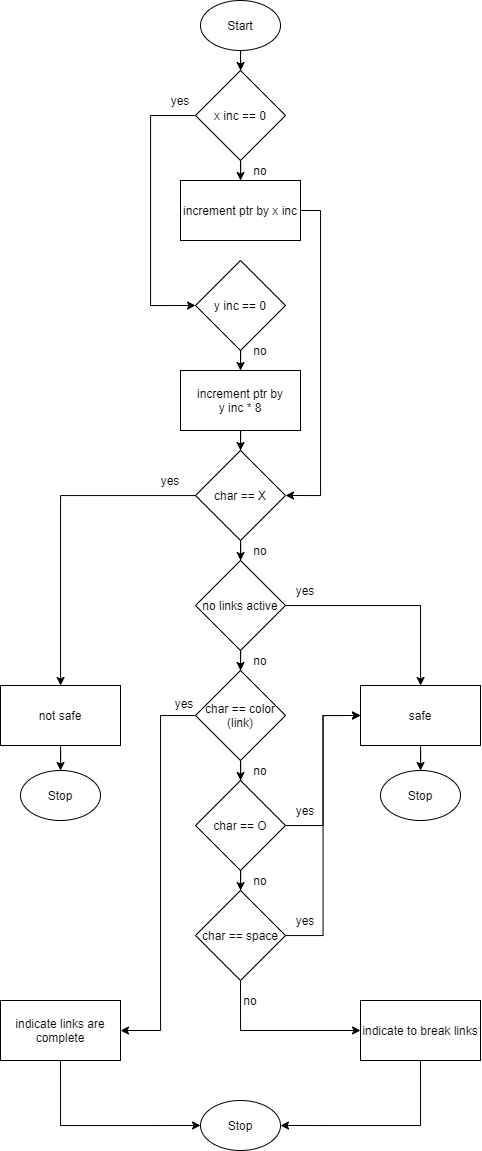
\includegraphics[height=16cm]{check_move.png}\centering} 
        \end{center}
        \newpage
        
    \subsubsection{check\_spot}
        This subroutine determines if the position is safe to put a link.
        If the current position is an O, you don't want to overwrite the 
        O with a link.
        \begin{center}
            {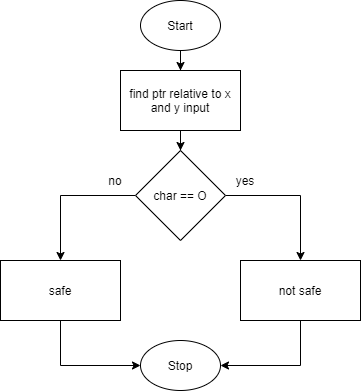
\includegraphics[height=7cm]{check_spot.png}\centering} 
        \end{center}
        \newpage

    \subsubsection{get\_subboard\_ptr}
        This routine takes in x and y coordinates and returns the subboard
        location replative to the input.
        \begin{center}
            {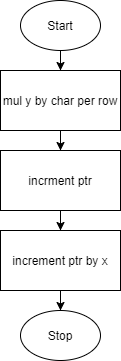
\includegraphics[height=5.5cm]{get_subboard_ptr.png}\centering} 
        \end{center}

    \subsubsection{place\_link}
        This subroutine takes a color 1-7 as an input at places the int as a 
        char into the subboard.
        \begin{center}
            {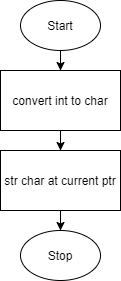
\includegraphics[height=4cm]{place_link.png}\centering} 
        \end{center}
        \newpage

    \subsubsection{get\_color}
        This routine is utilized when space is pressed to determine what
        the active color should be.  If no color is present it returns 0.
        \begin{center}
            {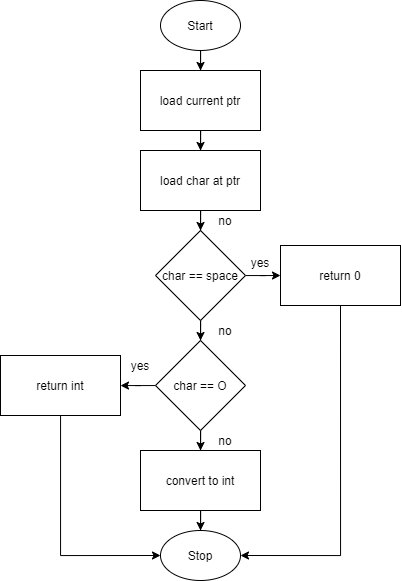
\includegraphics[height=9cm]{get_color.png}\centering} 
        \end{center}
        \newpage

    \subsubsection{get\_cursor\_pos}
        This subroutine gets the correct cursor position within
        the board relative to the inputs x and y.
        \begin{center}
            {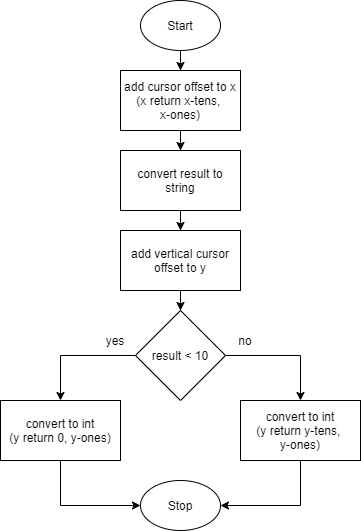
\includegraphics[height=8cm]{get_cursor_pos.png}\centering} 
        \end{center}
        \newpage

    \subsubsection{clear\_pos\_sub\_board}
        This subroutine moves to the ptr relative to x and y
        within the subboard and places a space into that position.
        \begin{center}
            {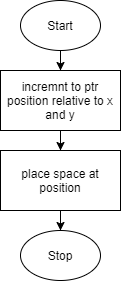
\includegraphics[height=4cm]{clear_pos_sub_board.png}\centering} 
        \end{center}

    \subsubsection{coord\_to\_byte}
        This routine encodes x and y coordintes to be store within 
        one byte.
        \begin{center}
            {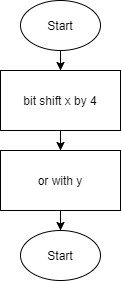
\includegraphics[height=4cm]{coord_to_byte.png}\centering} 
        \end{center}

    \subsubsection{byte\_to\_coord}
        This routine reverses the encoding to output x and y coordinates.
        \begin{center}
            {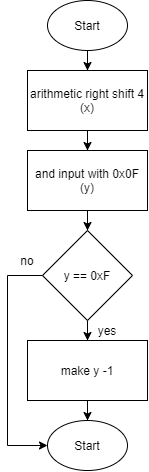
\includegraphics[height=6cm]{byte_to_coord.png}\centering} 
        \end{center}
        \newpage

    \subsubsection{check\_win}
        This subroutine determines if there are still any spaces on the board.
        If there are not, the board is completed.
        \begin{center}
            {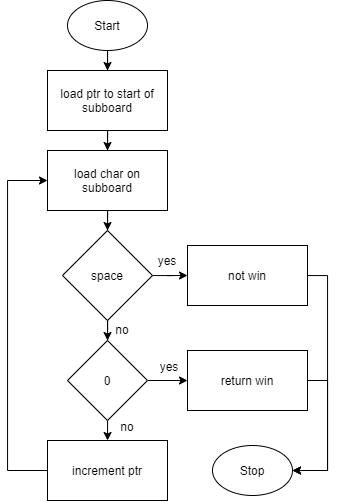
\includegraphics[height=8cm]{check_win.png}\centering} 
        \end{center}
        \newpage

    \subsubsection{last\_link}
        Theh routine is utilized when unpausing.  Due to the way link 
        coordinates are stored this routine is required to try to find
        the O that is nearby.
        \begin{center}
            {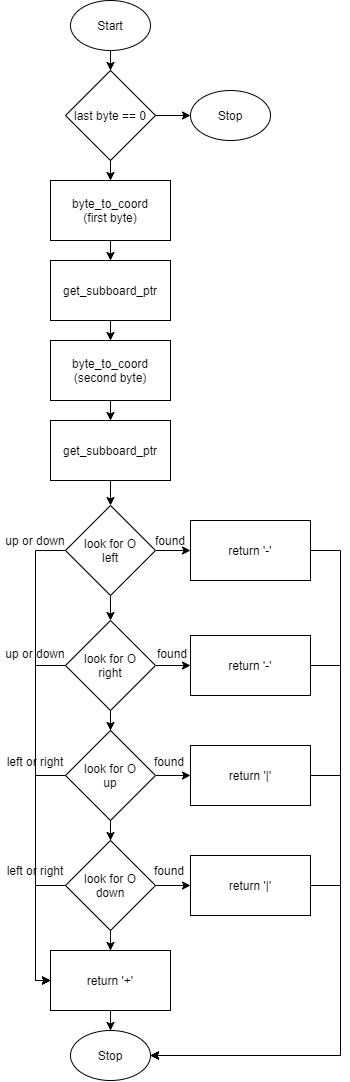
\includegraphics[height=14cm]{last_link.png}\centering} 
        \end{center}
        \newpage


\subsection{Complete.s}
    This file is responsible for incrementing or decrementing 
    the completed number or determining if the game has been won.
    Inorder to determine if a specific color link is allowed to 
    be changed 7 bytes of memory were used for each color.  If a 
    1 was in space 3 (blue-start at 0) that means that link was already completed.
    If it was 0 it means that there is no link and it can't be decremented.

    \subsubsection{modify\_completed}
    This subroutine determines if it is okay to increment or decrement 
    the completed number. The inputs are the number to increment by and
    the color that was been broken or completed.

    \begin{center}
        {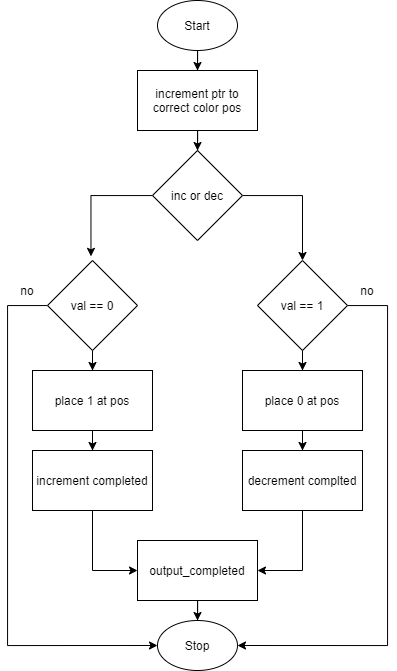
\includegraphics[height=8cm]{modify_completed.png}\centering} 
    \end{center}
    \newpage

    \subsubsection{output\_completed}
    This routine outputs the string for completed. The string contains both the 
    value for completed and the cursor position. It takes in an int for the 
    completed value and returns a 0 or 1 for game done.
    \begin{center}
        {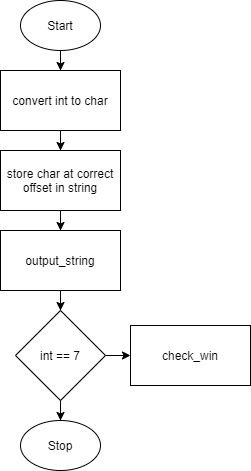
\includegraphics[height=6cm]{output_completed.png}\centering} 
    \end{center}

    \subsubsection{clear\_completed}
    This subroutine sets each byte in memory to 0 for the completed values.
    It also sets the completed int to 0.
    \begin{center}
        {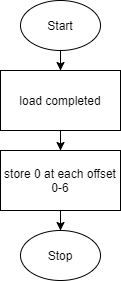
\includegraphics[height=5cm]{clear_completed.png}\centering} 
    \end{center}
    \newpage

    \subsubsection{check\_completed}
    This routine increment to the correct positon in memory
    and returns whether or not the input color link has been
    completed.
    \begin{center}
        {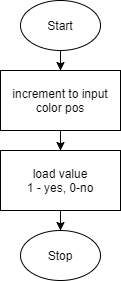
\includegraphics[height=4cm]{check_completed.png}\centering} 
    \end{center}

    \subsubsection{reprint\_completed}
    This subroutine reprints the completed string for cases where 
    the completed value does not need to be changed.
    \begin{center}
        {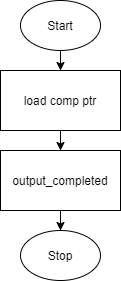
\includegraphics[height=4cm]{reprint_completed.png}\centering} 
    \end{center}
    \newpage


\subsection{Library.s}
    This file contains all of the generalized subroutines that we
    have made througout the semester.
    \subsubsection{read\_character}
        read\_character first sets the uart address then increments to the flag bit 
        for input. It loads the flag bit to determine if a key was pressed and if it
        was, then it loads the character.

        \begin{center}
            {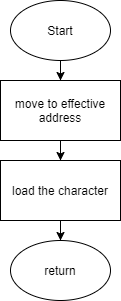
\includegraphics[height=5cm]{read_character.png}\centering} 
        \end{center}

    \newpage
    \subsubsection{output\_character}
        output\_character will output a character that is typed to the putty screen. This
        is done by moving to the uart adress and visting the flag bit. It isolates the flag bit and 
        stores its data (the character pressed).
        \begin{center}
            {\includegraphics[height=10cm]{output_char.png}\centering} 
        \end{center}


    \newpage
    \subsubsection{output\_string}
        output\_string is given a string and calls output\_character on each specific character on the string
        until it reaches a null character. When it reaches a null character the output\_string function stops.
        \begin{center}
            {\includegraphics[height=9cm]{output_string.png}\centering} 
        \end{center}


    \newpage
    \subsubsection{read\_string}
        read\_string calls read\_character to accept input and then output\_character
        to display the read character on the screen.  It continues to read until 
        the enter key is pressed and null terminates the string.
        \begin{center}
            {\includegraphics[height=10cm]{read_string.png}\centering} 
        \end{center}
    \newpage


    \subsubsection{uart\_init}
        Ths subroutine initializes the uart in order for it to be used. This is done by isolating specific
        peices of memory and storing a specific value at those peices of memory.

    \subsubsection{gpio\_init}
        This subroutine initializes the tiva board for use with gpioo
        \begin{center}
            {\includegraphics[height=6cm]{illuminate_RGB_LED.png}\centering} 
        \end{center}

    \newpage
    \subsubsection{read\_from\_push\_btn}
        This routine checks if the button is currently being pressed
        \begin{center}
            {\includegraphics[height=12cm]{read_from_push_btn.png}\centering} 
        \end{center}

    \newpage
    \subsubsection{illuminate\_RGB\_LED}
        This routine changes the color of the LEDs based on the input 1-7
        \begin{center}
            {\includegraphics[height=8cm]{illuminate_RGB_LED.png}\centering} 
        \end{center}

    \newpage
    \subsubsection{correct\_num}
        This routine will achange numbers taken from subroutines in Lab6 and make
        the number taken from the ANSI Escape Sequences and correctly correlate them
        to the number that needs to be passed into illuminate\_RGB\_LED.
        \begin{center}
            {\includegraphics[height=9cm]{correct_num.png}\centering} 
        \end{center}

    \newpage
    \subsubsection{num\_digits}
        num\_digits will calculate the number of digits in a string. This is done by
        dividing by 10 and incrementing the number of digits each time the divison is done until
        the int is equal to 0.

        \begin{center}
            {\includegraphics[height=12cm]{num_digits.png}\centering} 
        \end{center}

    \newpage
    \subsubsection{int2str}
        int2str will turn an integer value into a string and output that string. This is done by
        calculating the value at each digit in the int and then finding the ASCII value for that digit
        and storing that value. 

        \begin{center}
            {\includegraphics[height=17cm]{int2str.png}\centering} 
        \end{center}
    \newpage

    \newpage
    \subsubsection{str2int}
        str2int initializes a posistional register to 0 then loops through each character 
        until the null terminator. At each character it multiplies the posistional int by
        10 and subtracts 0x30 from the character to isolate the int. It adds that value
        to the return value and increments the posistional int.

        \begin{center}
            {\includegraphics[height=12cm]{str2int.png}\centering} 
        \end{center}

    \newpage
    \subsubsection{negate\_int}
        This routine performs a bit flip to negate the input number and
        adds 1.
        \begin{center}
            {\includegraphics[height=6cm]{negate_int.png}\centering} 
        \end{center}

\end{document}